\documentclass{article}
\usepackage{fullpage,amsmath,amsthm,graphicx,enumitem}
\usepackage{multicol}
\usepackage{booktabs}
\usepackage{hyperref}
\usepackage{tikz}

\theoremstyle{definition}
\newtheorem{thm}{Theorem}
\newtheorem{question}[thm]{Question}
\newenvironment{solution}{\noindent\textit{Solution:}}{}

\title{ASEN 6519: Optimization: Applications and Algorithms\\
       Homework 4}

\begin{document}

\begin{center}
{\large \textbf{ASEN 6519: Optimization: Applications and Algorithms} \\ \textbf{Homework 4}}\\
\end{center}

% \maketitle

\begin{question}(Lagrange Multipliers)

    Write your own implementation of a numerical algorithm such as the augmented Lagrangian or primal-dual interior-point method to find the Lagrange multipliers for the simple optimal control problem from question 3 of Homework 3. Write the constraints in the form $\mathbf{g}(\mathbf{x}) \leq 0$ and report values of the Lagrange multipliers for each element of the constraint function. You may use the homework 3 solutions and algorithms from the book as starting points.
\end{question}

\begin{question}(Sudoku)

    Pose Sudoku (\url{https://en.wikipedia.org/wiki/Sudoku}) as an optimization problem (or a constraint satisfaction problem) and solve it using an off-the-shelf optimizer. Note: since this is a classic problem, there are many tutorials online. You may look at them, but please take a stab at it before looking at them.
    Deliverables for this problem are (1) the mathematical formulation of the optimization problem, (2) the code you used to solve it, and (3) the solution to the problem in the image below from wikipedia:
    \begin{center}
        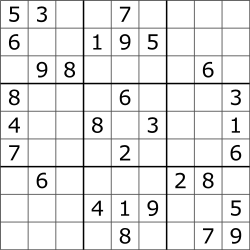
\includegraphics[width=0.2\textwidth]{sudoku.png}
    \end{center}
\end{question}

\begin{question}(Risk-aware portfolio design via nonlinear programming)

    Suppose that you are investing an initial sum of \$1000 in a portfolio of four assets (it is possible to purchase fractional shares).
    A share of each asset costs $c_i$ dollars and the value per share of each asset at the end of a year is a Gaussian random variable with mean $v_i$ and standard deviation $\sigma_i$. The profit is the value minus the initial cost. Data to copy and paste into your code is available in \texttt{hw4-data.txt}.
    \begin{enumerate}
        \item Formulate the problem of maximizing the expected value of the portfolio as a linear program and solve it with an off-the-shelf solver. How many shares of each asset should you buy, and what is the expected profit?
        \item Formulate a nonlinear program for maximizing the expected value of the portfolio subject to the constraint that the standard deviation of the profit is no more than half the expected profit. Solve the problem with an off-the-shelf solver. How many shares of each asset should you buy and what is the expected profit?
        \item Now suppose that a more complex model that captures correlations between the assets is available so that the value of the entire portfolio is a Gaussian random variable with mean $\mathbf{v}^\top \mathbf{x}$ and standard deviation $$\sigma = \sqrt{\mathbf{x}^\top \Sigma \mathbf{x}} \text{,}$$ where $\mathbf{x}$ is a vector of shares of each asset and $\Sigma$ is the covariance matrix. Formulate the problem of maximizing the expected value of the portfolio subject to the constraint that the standard deviation is no more than half the expected profit. Solve the problem with a nonlinear solver such as \texttt{Ipopt} or \texttt{fmincon} or code you have written yourself. How many shares of each asset should you buy and what is the expected profit?
        
        Bonus: do all of the assets in the optimal portfolio for part 3 have positive expected profit? If not, why are they part of the portfolio?
    \end{enumerate}
\end{question}

\end{document}
